%%%%%%%%%%%%%%%%%%%%%%%%%%%%%%%%%%%%%%%%%%%%%%%%%%%%%%%%%%%%%%%%%%%%%%%%%%%%%%%%
% experiment.tex: Chapter describing the experiment
%%%%%%%%%%%%%%%%%%%%%%%%%%%%%%%%%%%%%%%%%%%%%%%%%%%%%%%%%%%%%%%%%%%%%%%%%%%%%%%%
\chapter{Experiment}
\label{experiment_chapter}
%%%%%%%%%%%%%%%%%%%%%%%%%%%%%%%%%%%%%%%%%%%%%%%%%%%%%%%%%%%%%%%%%%%%%%%%%%%%%%%%
\subsection{The Large Hadron Collider}
\begin{itemize}
	\item need high energy and inst lumi to search for weakly coupled interactions with heavy mediating particles
	\item high energy and lumi drive dramatically increase rate of low energy and other abundant processes. explain these
	\item QCD multijet event rate at LHC is O(100 kHz), CMS readout capability is O(100 Hz) $\rightarrow$ need fast, efficient trigger system
	\item describe 2015 run conditions - cause of PU, PU range observed in data, consequences on trigger, offline reco and analysis
\end{itemize}
Situated near Geneva Switzerland, the Large Hadron Collider (LHC) is the highest energy particle
collider in the world.  Operated by the European Organization for Nuclear Research (CERN), the LHC resides in
a 27 km circumference tunnel previously used for the Large Electron Positron Collider (LEP).  Collisions between
protons in the LHC begin with low energy hydrogen atoms.  Hydrogen gas is heated into a plasma from which protons are
extracted.  Protons then travel through several accelerator stages, gaining energy after every stage, and end in
the LHC.  In the LHC, strong magnetic and electric fields created by superconducting magnets and RF cavities 
create two collimated beams of high energy protons which collide at four interaction points.  The LHC was
designed to accelerate both beams of protons such that collisions occur at a center of mass energy of 14 TeV,
initially at an instantaneous luminosity of $2x10^{33} \frac{1}{cm^{2}s}$ \cite{}.  After a few years of successful running
the instantaneous luminosity would increase.

%why are high lumi and energy needed
The LHC was built to discover new physics mediated by heavy particles which are weakly coupled to Standard Model (SM)
leptons, hadrons and bosons.  To produce heavy, weakly interacting particles, like a $2.0 TeV$ mass right handed W ($W_{R}$) boson
with production cross section 5 fb, at a rate sufficient for detection, average instantaneous luminosities of
$10^{33} \frac{1}{cm^{2}s}$ are needed.  At such luminosities, other more abundant or lower energy processes will occur
at a significant rate, as shown in Figure \ref{smProductionXsxns}.

Of all processes created by collisions in the LHC, low energy, inelastic QCD interactions occur at the highest rate, of the order
$10^{8}$ events per second at $10^{33} \frac{1}{cm^{2}s}$.  Contributions from these events to new physics searches are mitigated by vetoing
on large groups of particles collinear with the beam line, or requiring the presence of leptons or photons.  However, these
requirements are not sufficient to suppress leptonic backgrounds created by the production and decay of heavy quarks, and QCD multijet
events in which a jet is incorrectly reconstructed as a lepton due to energetic neutral pions in the jet.  Such high energy QCD multijet
and heavy quark decay events occur at a rate of $10^{5}$ events per second at $10^{33} \frac{1}{cm^{2}s}$.  These event rates dwarf
the rate at which entire events can be read out of CMS and saved to disk, approximately $10^{3}$ events per second.  The tools, generally
called triggers, used to select and save collision events at a tolerable rate will be discussed later.

\begin{figure}[h]
	\centering
	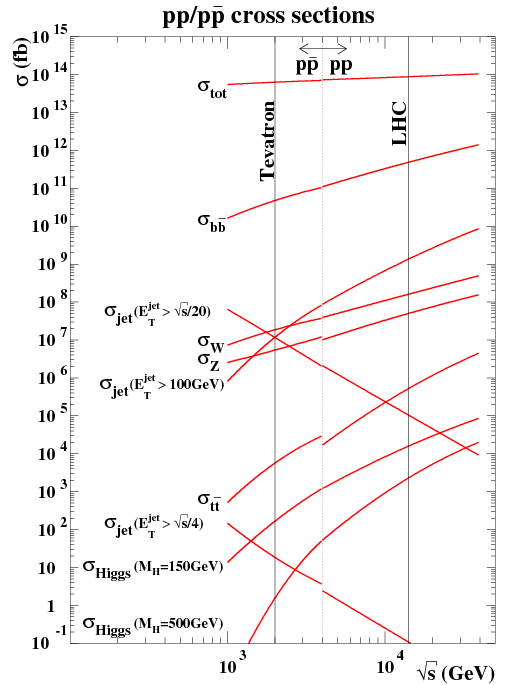
\includegraphics[width=0.6\textwidth]{figures/lhc_and_tevatron_cross_sections_2006.png}
	\caption{Production cross sections at the LHC and Tevatron as a function of center of mass energy. \cite{}}
	\label{fig:smProductionXsxns}
\end{figure}


%Operations
The LHC started operations with collisions at a lower center of mass energy and lower instantaneous luminosity than design.  In 2015 the center of mass
energy was increased to 13 TeV, and the luminosity was increased closer to the design level.  The 2015 data taking period was split into two portions - from the start
of 2015 collisions until August the time separation between consecutive proton bunches in each beam was 50 ns.  After August, the bunch
separation decreased to 25 ns, and proton proton collisions continued until November.  During this time, instantaneous luminosities reached $5x10^{33} \frac{1}{cm^{2}s}$, but
problems with the CMS magnet cooling system limited the amount of data collected to 2.6 $fb^{-1}$.

At 13.



\subsection{Compact Muon Solenoid Detector Overview}
\begin{itemize}
	\item general design goals which ultimately focus down to WR search
	\item brief description of each subdetector and magnet
	\item trigger description, followed by particle flow event reconstruction
\end{itemize}

\subsection{Track and vertex reconstruction}

\subsection{Muon Reconstruction and Identification}
\begin{itemize}
	\item importance of muons, challenges with reco and energy measurements
	\item muon detector technologies
	\item muon reconstruction algorithms
	\item challenge with pT measurement of high pT muons
	\item explain TuneP algorithm and show performance plots
	\item explain ID variables, isHighPt ID and show performance plots
	\item explain usefulness of muon isolation (reject muons from QCD) and how it is calculated
	\item muon L1 and HLT: design and performance plots
\end{itemize}

\subsection{Electron Reconstruction and Identification}
\begin{itemize}
	\item importance of electrons, challenges with reco and energy measurements
	\item ECAL
	\item electron reconstruction algorithms
	\item challenge with pT measurement of high pT muons
	\item explain TuneP algorithm and show performance plots
	\item explain ID variables, HEEP ID and show performance plots
	\item explain usefulness of electron isolation (reject eles from QCD) and how it is calculated
	\item electron L1 and HLT: design and performance plots
\end{itemize}



\subsection{Particle Flow and Jet Reconstruction}



